\PassOptionsToPackage{quiet}{fontspec}
\documentclass[12pt,a4paper]{article}
\usepackage{thesis} % 格式控制
\usepackage{indentfirst}
\usepackage{enumitem}
\usepackage{amsmath} % 数学公式支持
\usepackage{amsfonts} % 数学字体支持
\usepackage{amssymb} % 数学符号支持
\usepackage{graphicx} % 图片插入支持
\usepackage{float} % 浮动体位置控制，支持 [H] 选项
\usepackage{caption} % 图表标题格式控制
\usepackage{geometry} % 页面布局控制
\usepackage{setspace} % 行距控制
\usepackage{xeCJK} % 中文字体支持
\usepackage{fontspec} % 字体设置
\usepackage[most]{tcolorbox} % 高亮按键命令
\usepackage{listings} % 代码高亮
\usepackage[table]{xcolor} % 颜色支持
\setlength{\parindent}{2em} % 控制首行缩进  
\addtolength{\parskip}{3pt} % 控制段落距离  
\onehalfspacing % 1.5倍行距  
\graphicspath{{./figures/}} % 指定图片所在文件夹  
\setCJKmainfont{SimSun}

% 配置lstlisting样式
\lstset{
    basicstyle=\ttfamily\small,
    breaklines=true,
    frame=single,
    numbers=left,
    numberstyle=\tiny\color{gray},
    backgroundcolor=\color{gray!10},
    keywordstyle=\color{blue},
    commentstyle=\color{green!60!black},
    stringstyle=\color{red},
    showstringspaces=false,
    tabsize=4,
    captionpos=b,
    xleftmargin=2em,
    xrightmargin=2em,
    aboveskip=1em,
    belowskip=1em
}

\classname{\heiti\bfseries 信息电子学物理基础}  % 设置课程名称
\makepagestyle{}{}

\newtcbox{\keyblue}{on line,
  colframe=blue!60!black, colback=blue!5,
  boxrule=0.8pt, arc=2pt, boxsep=0pt, left=3pt, right=3pt, top=2pt, bottom=2pt,
  tcbox raise base, fontupper=\ttfamily\small}

\newtcbox{\pathbox}{on line,
  colframe=green!60!black, colback=green!5,
  boxrule=0.8pt, arc=2pt, boxsep=0pt, left=3pt, right=3pt, top=2pt, bottom=2pt,
  tcbox raise base, fontupper=\ttfamily\small}

\begin{document}
\maketitlepage{耿氏二极管初步设计}{玉泉教7-104}{}{}{\today}{林时胜} %封面页 

\maketoc

\section*{摘要}
本设计提出基于自对准阳极场板的三端异形沟道平面耿氏二极管（3T-GS-PGD），突破 GaN 耿氏器件"雪崩先于振荡"瓶颈。核心创新在于：自对准场板消除阳极侧电场热点，底部控制极 $V_S$ 夹断漏电流路径，T 型沟道降低启动电压至 10--20 V，实现 >300 GHz 稳定振荡。该方案兼顾电学性能与工艺可行性，为 THz 固态振荡源提供完整技术路径。

\section{设计背景与目标}

\subsection{太赫兹（THz）技术及其应用}

太赫兹（THz）波通常指频率在0.1 THz到10 THz（波长3mm到30µm）范围内的电磁波。这一波段位于传统电子学（毫米波）和光子学（红外线）之间，被称为"太赫兹鸿沟"（THz Gap）。

\begin{table}[H]
    \centering
    \caption{电磁波谱中太赫兹波段的位置}
    \begin{tabular}{lcc}
        \toprule
        \textbf{名称} & \textbf{波长} & \textbf{频率} \\
        \midrule
        无线电波 & 3000m--10mm & 10KHz--30GHz \\
        毫米波 & 10mm--1mm & 30--300GHz \\
        亚毫米波 & 1mm--100µm & 300GHz--3THz \\
        \rowcolor{blue!10} 太赫兹 & 3mm--30µm & 100GHz--10THz \\
        红外线 & 1mm--760nm & 300GHz--430THz \\
        可见光 & 760nm--400nm & 430--790THz \\
        \bottomrule
    \end{tabular}
\end{table}

THz技术在医疗成像、生物检测、安全检查、高速通信、航空航天工业等领域具有巨大的应用潜力\cite{tonouchi2007cutting}\cite{siegel2004terahertz}。

\subsection{现有技术瓶颈}

目前，实现高效、紧凑、室温工作的THz震荡源是该领域面临的主要挑战：

\begin{itemize}
    \item \textbf{电子学方案：}传统的晶体管等电子器件在高频（>300 GHz）下性能严重下降。
    \item \textbf{光子学方案：}例如量子级联激光器（QCLs），虽然可以产生THz波，但通常系统庞大、操作复杂，且许多设备仅在低温制冷条件下才能工作，不适用于大规模消费级应用\cite{belkin2007terahertz}。
\end{itemize}

因此，开发在室温下工作、结构紧凑、成本低廉的电子学THz发射源，是推动THz技术广泛应用的迫切需求。耿氏二极管（Gunn Diode）作为一种有源两端器件，是实现这一目标的有力候选者。

\subsection{本设计目标}

本项目旨在设计并论证一款基于自对准阳极场板的三端异形沟道平面耿氏二极管（3T-GS-PGD）。其核心目标是：

\begin{itemize}
    \item \textbf{突破性创新：}针对GaN耿氏二极管"雪崩先于振荡"的核心瓶颈，提出\textbf{自对准阳极场板}方案从根本上消除阳极侧沟槽边缘的电场热点；配合三端结构中的底部控制极$V_S$夹断漏电流路径，实现"高场振荡"与"雪崩抑制"的安全解耦。
    \item \textbf{高性能目标：}采用掺杂GaN有源层和T型沟道几何结构，设计沟道长度$L = 0.5$ µm，使振荡频率进入太赫兹波段（目标频率 $f = 500$ GHz，即 > 300 GHz），工作电压控制在10--20 V范围内。
    \item \textbf{工程可行性：}充分考虑MOCVD外延生长、光刻工艺、热管理（SiC衬底）等制造工艺要求，自对准阳极场板方案简化制造难度，提高器件可靠性。
    \item \textbf{安全与社会责任：}全面评估生产制造过程中的安全防护需求（剧毒气体、强酸腐蚀）、环境影响（废气废水处理）以及技术应用的社会效益（6G通信、医疗成像、安全检查），确保设计符合可持续发展原则。
\end{itemize}

\clearpage
\section{耿氏二极管基本原理}

\subsection{耿氏效应}

耿氏二极管（Gunn diode）属于转移电子器件（Transfer Electron Device, TED），
其工作原理不是基于PN结整流，而是利用某些半导体在高电场下出现的负微分电阻（Negative Differential Resistance, NDR）现象。
典型具有NDR的材料包括GaAs、InP以及GaN等，它们在导带上存在迁移率高的低能谷，称为中心能谷（$\Gamma$-valley）和迁移率较低的高能谷,称为卫星能谷（Satellite L-valley）。

\begin{figure}[H]
    \centering
    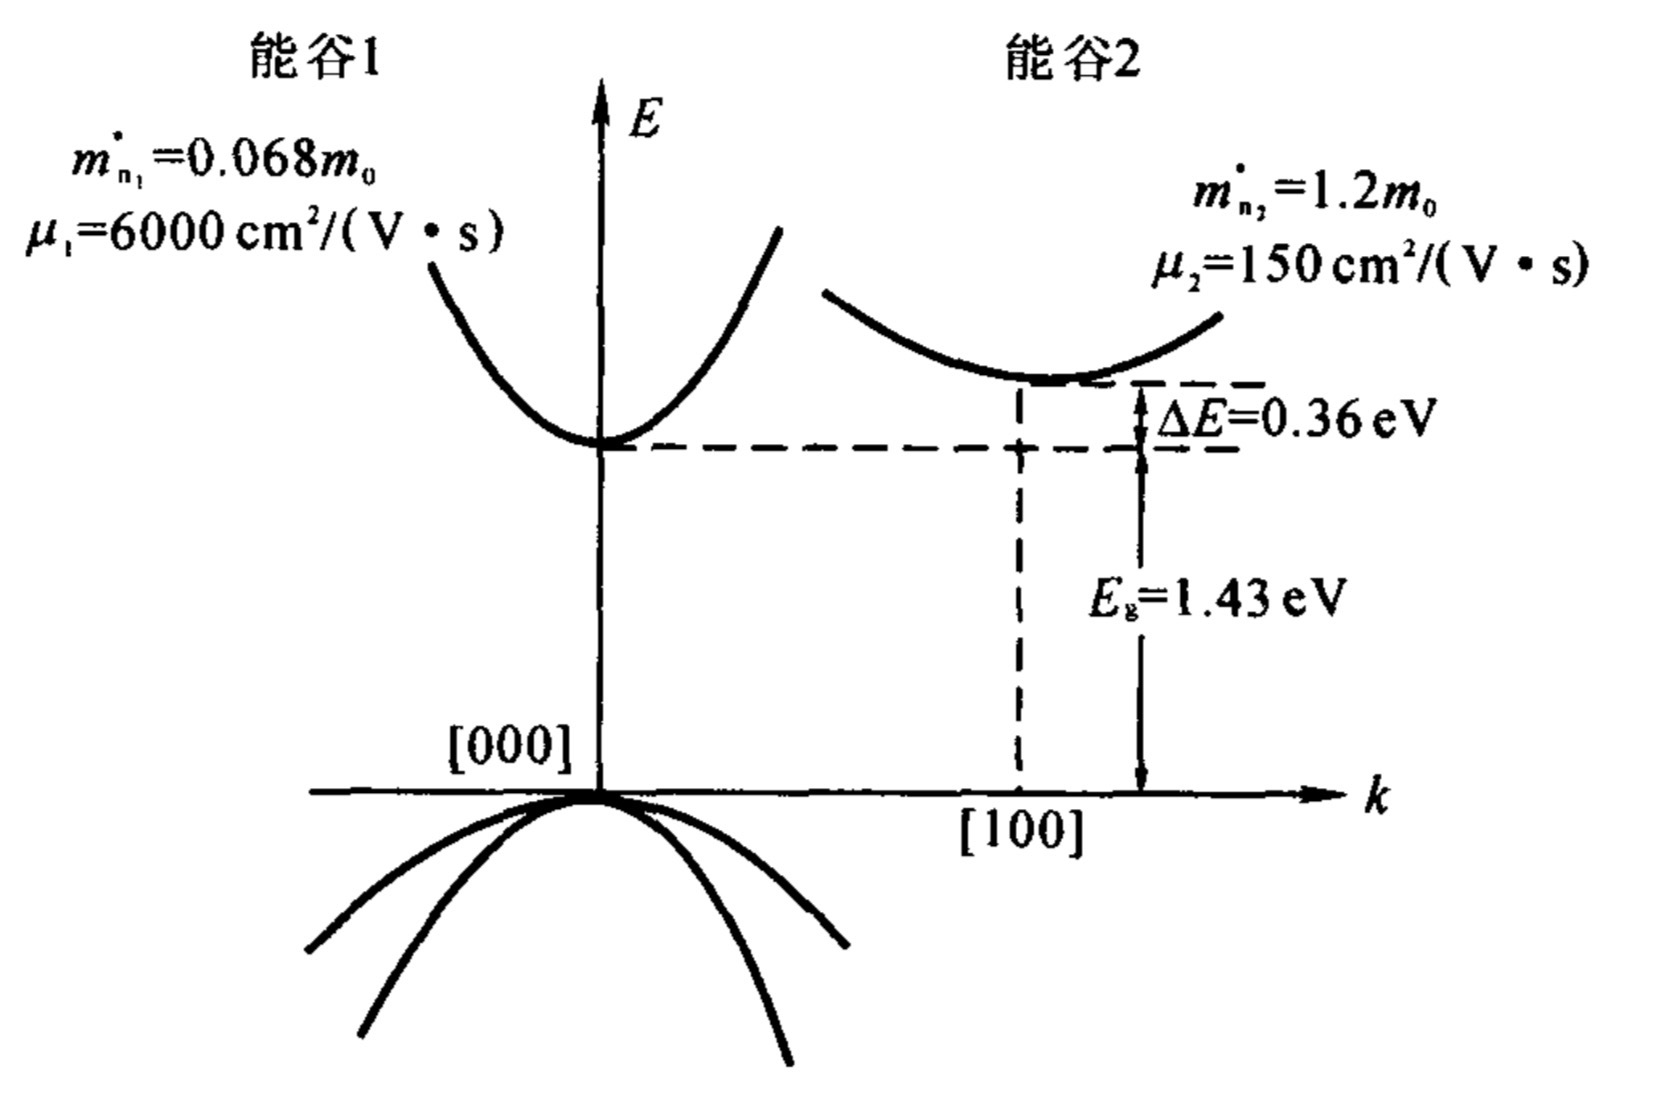
\includegraphics[width=0.5\textwidth]{p2.jpg}
    \caption{能谷示意图}
\end{figure}
当给像 GaN 这样导带具有双能谷的半导体两端施加电压时，低能谷高迁移率的电子在电场的作用下向高能谷转移，称为转移电子效应（耿氏效应）。转移电子效应的结果是产生了负微分电阻（NDR），规定低能谷的电子迁移率和电子密度分别为 $\mu_1$ 和 $n_1$，高能谷的电子迁移率和电子密度分别为 $\mu_2$ 和 $n_2$。半导体电流密度为：

\begin{equation}
    J = q(\mu_1 n_1 + \mu_2 n_2)\varepsilon = qnv
\end{equation}

其中 $v$ 为平均漂移速度：

\begin{equation}
    v = \left(\frac{\mu_1 n_1 + \mu_2 n_2}{n_1 + n_2}\right)\varepsilon \approx \frac{\mu_1 \varepsilon}{1 + \left(\frac{n_2}{n_1}\right)}
\end{equation}

高低能谷之间的电子数目比为：

\begin{equation}
    \frac{n_2}{n_1} = \exp\left(\frac{-\Delta E}{kT_e}\right)
\end{equation}

得到速度-电场关系为：

\begin{equation}
    v = \mu_1 \varepsilon \left[1 + \exp\left(-\frac{\Delta E}{kT_e}\right)\right]^{-1}
\end{equation}

\begin{equation}
    \mu_2 < \mu_1
\end{equation}

根据以上公式，刚加上电场时，由低能谷转移到高能谷的电子很少，此时总的电子密度大约等于低能谷电子密度，电流主要取决于低能谷电子。随着电场的增加，电流增加。当电场继续增大时，高能谷的电子密度远远大于低能谷，高能谷的电子密度起主要作用，又因其迁移率小于低能谷电子的迁移率，所以总电流降低，出现负微分电阻。

\begin{figure}[H]
    \centering
    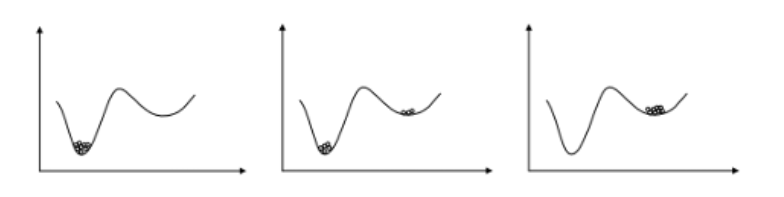
\includegraphics[width=0.8\textwidth]{p3.png}
    \caption{电子能谷转移示意图\cite{yao2014thz}}
\end{figure}

\subsection{耿氏畴的形成}

在低电场下，电子主要分布在低能谷，迁移率和漂移速度随电场近似线性增加；当电场超过阈值时，部分电子被加热并跃迁到高能谷，因而平均迁移率下降，导致电流随电场增加而下降（即出现NDR）。该过程在速度-电场曲线上表现为峰值速度后下降的区域。


图(a)表示漂移电流密度 $J$ 与电场 $E_{\text{场}}$ 的关系，图中存在明显的负阻区。图(b)是外加偏置电场
$E_{\text{场A}}$ 的两端器件。若在阴极附近，出现电子浓度一个涨落，于是形成图(c)所示偶极层，称为高场畴。

它所形成的场与外场方向相同。层内相对于层外，电场增强。层的左方和右方区域为低场区，分别处于 $E_{\text{场C}}$ 和 $E_{\text{场B}}$。高场畴稳定情况下，器件内的电场如图3.6.4(d)所示。畴内电子将以恒一漂移速度 $v_S$ 向阳极移动，到达阳极并从阳极"退出"，从而可以得到输出电流。同时，半导体内又处于外偏电场 $E_{\text{场A}}$，在阴极端附近新生长出一个高场畴并向阳极移动，又可输出电流脉冲。

\begin{figure}[H]
    \centering
    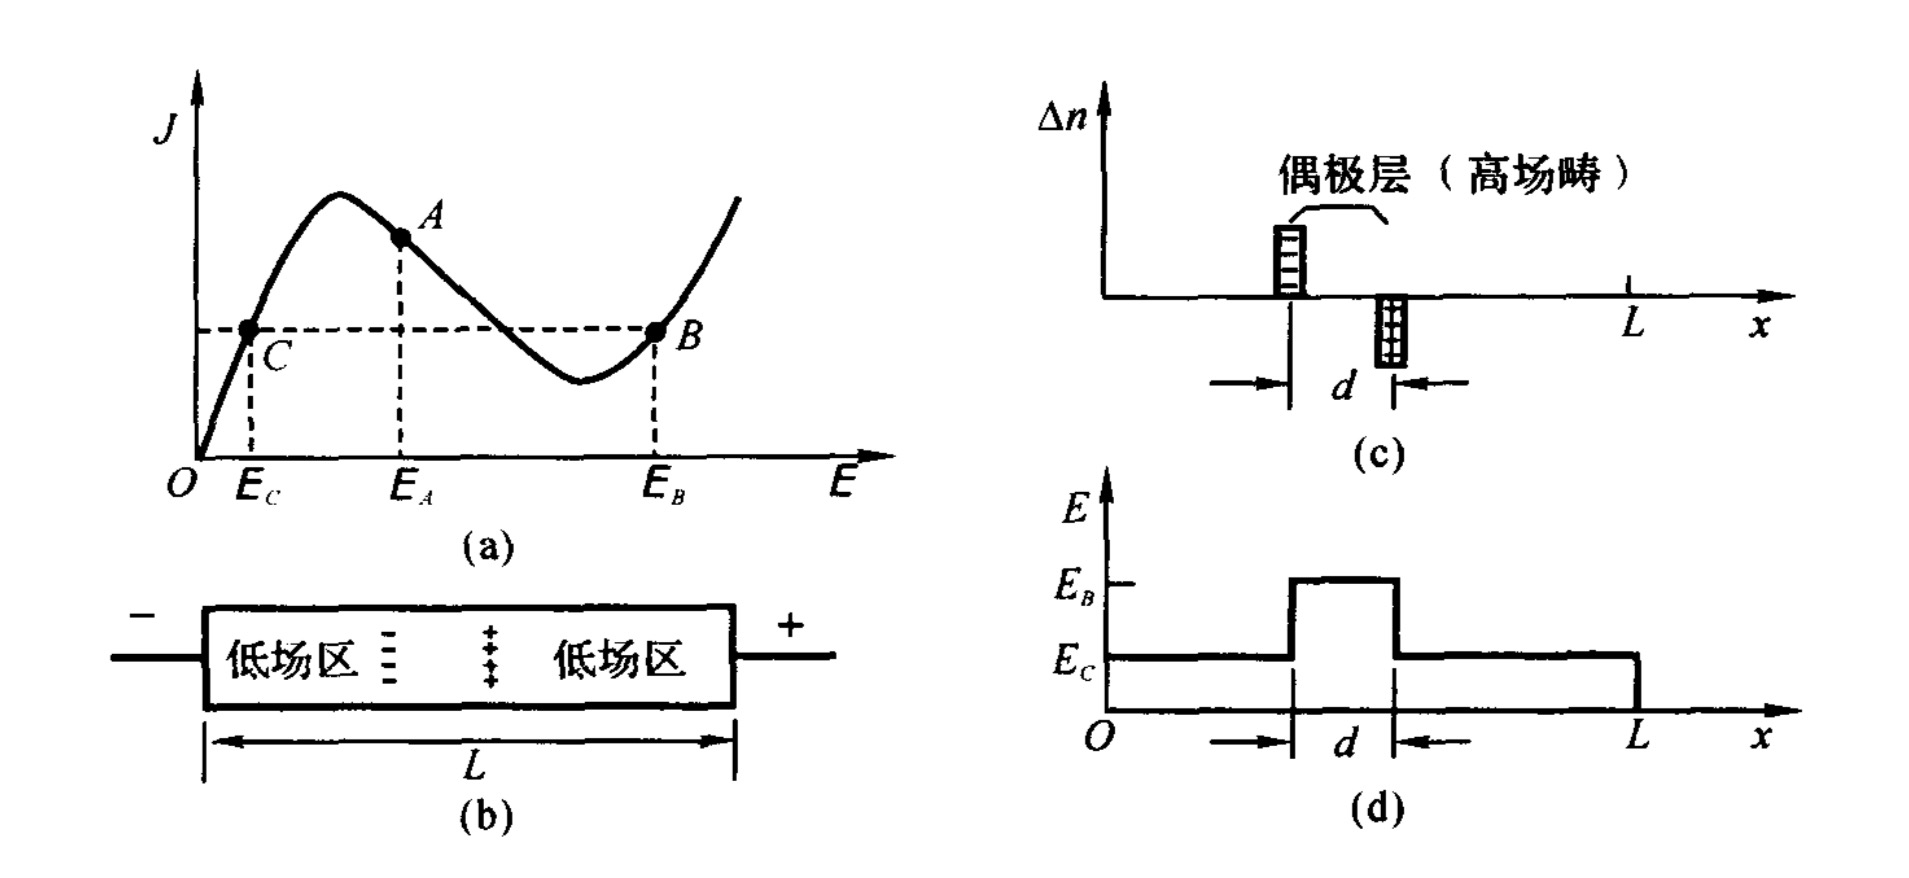
\includegraphics[width=0.8\textwidth]{p1.jpg}
    \caption{耿氏畴形成过程示意图}
\end{figure}

\subsection{耿氏二极管的震荡条件}

如上节所述，当阴极附近出现电子浓度涨落时，会形成高场畴（耿氏畴）并向阳极移动。这种畴的周期性形成与传播是耿氏二极管产生振荡的关键机制。然而，并非所有具有负微分电阻特性的器件都能产生稳定振荡，还需要满足特定的物理条件和几何条件。

\subsubsection{振荡的物理过程}

前文已经描述了高场畴以饱和漂移速度 $v_s$（约 $10^7$ cm/s）向阳极移动的过程。在此基础上，振荡的周期性产生机制如下：

\begin{itemize}
    \item 当畴形成并漂移时，它"吸收"了器件的大部分电压，导致器件外部的电场下降到阈值 $E_{th}$ 以下，阻止了新畴的形成。
    \item 当畴漂移到达阳极并消失时，器件内的电场重新上升到 $E_{th}$ 以上。
    \item 一个新的畴在阴极端附近重新形成，开始下一次循环。
    \item 这个循环过程导致外部电路中的电流产生周期性的脉冲，形成振荡。
\end{itemize}

\textbf{振荡频率（渡越时间模式）：}如果器件长度为 $L$，畴的漂移时间（渡越时间）为 $\tau_T = L/v_s$。因此，振荡的基准频率 $f_T$ 由渡越时间决定：

\begin{equation}
    f_T = \frac{1}{\tau_T} = \frac{v_s}{L}
\end{equation}

例如，一个 $L = 10\mu$m 的GaAs器件，其频率约为 $f_T \approx (10^7 \text{ cm/s})/(10 \times 10^{-4} \text{ cm}) = 10^{10}$ Hz = 10 GHz。

\subsubsection{产生振荡的两个充要条件}

综合以上推导，耿氏二极管要产生振荡，必须满足两个条件：

\textbf{1. 物理条件：}负微分迁移率（NDM）器件材料必须具有RWH效应（如GaAs），并且偏置电压必须使其内部电场 $E$ 处于 $v - E$ 曲线的下降区域。

\begin{equation}
    \mu_d = \frac{dv}{dE} < 0
\end{equation}

\textbf{2. 器件条件：}Kroemer 准则（nL 乘积）电荷扰动必须在它漂移出器件之前有足够的时间增长为成熟的"畴"。这意味着电荷的增长时间（即介电弛豫时间 $|\tau_r|$）必须远小于电子的渡越时间 $\tau_T$。

\begin{equation}
    \tau_T \gg |\tau_r|
\end{equation}

\begin{equation}
    \frac{L}{v_s} \gg \frac{\varepsilon}{qn_0|\mu_d|}
\end{equation}

重新整理，我们得到一个关于载流子浓度-长度乘积（$n_0L$）的准则：

\begin{equation}
    n_0L \gg \frac{\varepsilon v_s}{q|\mu_d|}
\end{equation}

对于 GaN 材料，这个临界值约在 $10^{13}$ cm$^{-2}$。


\begin{equation}
    n_0L > (n_0L)_{\text{crit}} \approx 10^{13} \text{ cm}^{-2} \quad \text{(for GaN)}
\end{equation}

如果 $n_0L$ 乘积小于这个值，器件虽然仍有NDM（负电阻），但畴来不及形成就会消出，因此它不会自发振荡，此时它可以用作一个（稳定的）微波放大器。

\clearpage
\section{GaN 材料选择}

GaN（氮化镓）作为一种第三代宽禁带半导体材料，在近年来的半导体技术中引起了广泛关注。与传统的硅（Si）和砷化镓（GaAs）等半导体材料相比，GaN 在高功率、高频率、以及高温和恶劣环境下的性能上具有显著的优势。GaN 的禁带宽度达到 3.4 eV，这使其在极端条件下表现出卓越的稳定性，尤其适用于高频和高功率应用，如射频（RF）功率放大器、激光器、以及高温和高电压设备等。

GaN 材料的崛起主要得益于其在电子和光电领域的独特优势。首先，GaN 具有非常高的热导率，使得基于 GaN 的器件能够更有效地散热，从而提高功率密度和器件的长期稳定性。此外，GaN 的临界击穿电场强度较高，达到 3.3 MV/cm，相比于 Si 和 GaAs，GaN 能够承受更高的电压，适合用于大功率、高电压的应用。

\subsection{GaN 能带结构}

GaN 的能带结构对其电子传输特性至关重要。如下图所示，GaN 在导带中存在多个能谷：中心 [000] 处存在最低能谷（Γ谷），大量的电子处于这个能谷中；在 [111] 方向存在次能谷。

\begin{figure}[H]
    \centering
    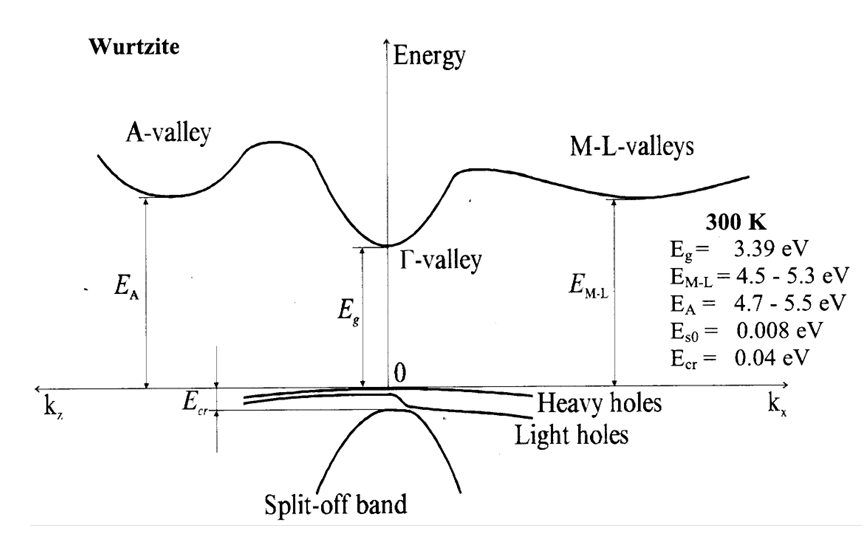
\includegraphics[width=0.7\textwidth]{p25.png}
    \caption{GaN 结构能带结构示意图，显示了Γ谷、卫星谷及各能级参数\cite{suzuki1995first}}
\end{figure}

\subsection{GaN 的优势与选择理由}

为了实现更高的工作频率和功率，本项目选择氮化镓（GaN）作为器件的有源材料。GaN 属于第三代宽禁带半导体，具有显著优势。

下面给出 GaN 与其他常见半导体材料的关键参数对比表（详见表）。

\begin{table}[H]
    \centering
    \caption{GaN与其他半导体材料关键参数对比\cite{li2018gan}}
    \begin{tabular}{lcccc}
        \toprule
        \textbf{参数} & \textbf{Si} & \textbf{GaAs} & \textbf{4H-SiC} & \textbf{GaN} \\
        \midrule
        禁带宽度（eV） & 1.12 & 1.42 & 3.25 & \textbf{3.45} \\
        电子饱和速度（$10^7$cm/s） & 1.0 & 2.0 & 2.0 & \textbf{2.7} \\
        电子迁移率（cm$^2$/V·s） & 1400 & 8500 & 1020 & 1000 \\
        相对介电常数 & 11.4 & 13.1 & 9.7 & 8.9 \\
        击穿场强（MV/cm） & 0.3 & 0.4 & 3.0 & \textbf{3.3} \\
        热导率（W/cm·K） & 1.5 & 0.5 & 4.9 & 2.0 \\
        \midrule
        Baliga优值（高频） & 1 & 11 & 73 & \textbf{180} \\
        Baliga优值（低频） & 1 & 16 & 600 & \textbf{1450} \\
        \bottomrule
    \end{tabular}
\end{table}

依据上表的材料参数对比，可以看出：

\begin{itemize}
    \item \textbf{禁带宽度：}GaN 的禁带宽度为 3.45 eV，能够有效抑制热激发的载流子，极大提高了在高温环境下的稳定性，使其特别适用于高温和高功率设备。
    \item \textbf{高电子饱和速度和速度：}GaN 的电子饱和速度为 $2.7 \times 10^7$ cm/s，比硅和砷化镓的速度高出许多，这使得 GaN 器件在保持较好的功率特性的同时，能够在高频和微波频段工作。
    \item \textbf{高击穿场强：}GaN 的临界击穿电场强度为 3.3 MV/cm，远高于 Si 和 GaAs 的击穿电场强度。这使得 GaN 器件在同等尺寸下能够承受更大的电压和电流，从而提高了器件的功率处理能力。
    \item \textbf{热导率：}GaN 的热导率为 2.0 W/cm·K，虽然略低于 SiC 的 4.9 W/cm·K，但仍显著高于 GaAs 的 0.5 W/cm·K。这一特点使得基于 GaN 的器件能够更有效地散热，从而提高功率密度和器件的长期稳定性。
    \item \textbf{较小的介电常数：}GaN 的相对介电常数为 8.9，相比于 Si 和 GaAs 较小，因此 GaN 器件的 PN 结电容较小，使得其更适用于高频应用。
\end{itemize}

此外，表中的 \textbf{Baliga 优值}（高频和低频）是衡量功率器件性能的重要指标。GaN 在高频应用中的 Baliga 优值达到 180，在低频应用中更是高达 1450，均显著优于传统的 Si、GaAs 等材料。这表明 GaN 在高频、高功率的应用场景中，具有独特的竞争力。

综上所述，GaN 作为一种第三代宽禁带半导体材料，其在高功率、高频率以及高温和恶劣环境下的优异性能，使得其成为现代电子器件中不可或缺的关键材料。

\clearpage
\section{GaN 耿氏二极管设计}

\subsection{GaN 耿氏二极管研究现状}

\subsubsection{耿氏二极管的两种实现形式}

根据电流流动方向和器件结构，GaN 耿氏二极管主要分为两类：垂直型（Vertical Device）和横向型/平面型（Lateral Device）。两种结构各有特点，适用于不同的应用场景。
下表总结了两种结构的对比：

\begin{table}[H]
    \centering
    \caption{横向与纵向GaN耿氏二极管结构对比}
    \begin{tabular}{p{2.5cm}p{5.5cm}p{5.5cm}}
        \toprule
        \textbf{特性} & \textbf{横向器件 (Lateral Device)} & \textbf{纵向器件 (Vertical Device)} \\
        \midrule
        \textbf{电极位置} & 源极、栅极、漏极都在芯片顶部 & 源极和栅极在顶部，漏极在底部 \\
        \midrule
        \textbf{电流路径} & 在AlGaN/GaN交界面的2DEG通道横向流动 & 垂直流动，从顶部经沟道穿过漂移区到底部 \\
        \midrule
        \textbf{承受电压} & 由栅极和漏极之间的横向距离决定 & 由垂直漂移区的厚度决定 \\
        \midrule
        \textbf{耿氏二极管结构} & 平面型（PGD），阴极和阳极在同一平面 & 垂直型，结构为$n^+/n/n^+$ \\
        \midrule
        \textbf{频率控制} & 由沟道长度（L）决定，可通过光刻精确控制 & 由中间$n$层厚度决定，外延生长后即固定 \\
        \midrule
        \textbf{优点} & $\bullet$ 工艺成熟，主流结构\newline $\bullet$ 频率灵活可调\newline $\bullet$ 易实现亚微米级短沟道（高频） & $\bullet$ 高耐压（几千伏）\newline $\bullet$ 面积效率高\newline $\bullet$ 适合高压大功率应用 \\
        \midrule
        \textbf{缺点} & $\bullet$ 提高耐压需增大间距\newline $\bullet$ 芯片面积增加\newline $\bullet$ 高压下效率受限 & $\bullet$ 制造工艺复杂\newline $\bullet$ 频率灵活性差\newline $\bullet$ 技术仍在发展中 \\
        \bottomrule
    \end{tabular}
\end{table}

\begin{figure}[H]
    \centering
    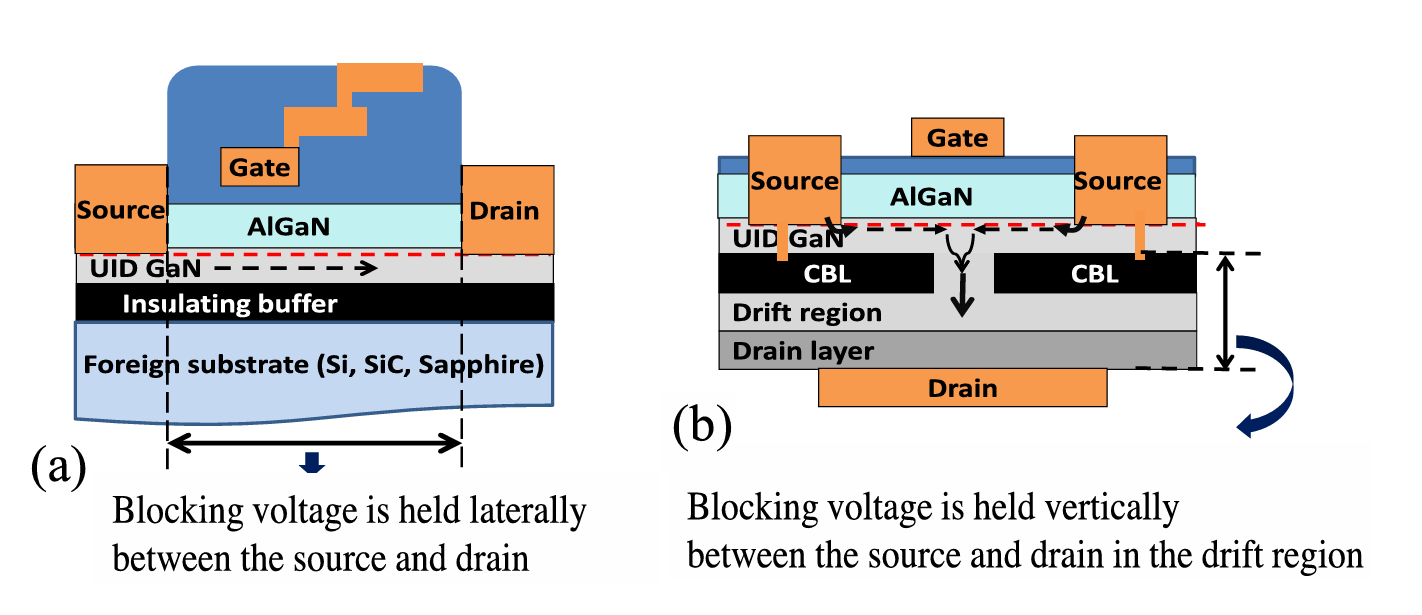
\includegraphics[width=0.9\textwidth]{p24.png}
    \caption{横向与纵向GaN器件结构对比示意图\cite{chowdhury2013lateral}}
\end{figure}

\subsubsection{GaN耿氏二极管的研究难点}

尽管GaN材料凭借其高电子饱和速度（$2.7 \times 10^7$ cm/s）、高击穿场强（3.3 MV/cm）和高Baliga优值等优势\cite{li2018gan}，被认为是实现高功率THz振荡源的理想选择，但在实际研究中，制造可靠的GaN耿氏二极管仍面临四大核心挑战：

\begin{itemize}
    \item \textbf{极高的启动电场（High Threshold Field）：} GaN的宽禁带（3.45 eV）和高能谷间距特性，导致其触发转移电子效应（NDR）所需的电场阈值（$E_{th}$）远高于传统的GaAs材料。这不仅意味着器件需要极高的工作电压，也对器件的稳定性和功耗提出了严峻的考验。

    \item \textbf{严重的自热效应（Severe Self-Heating Effect）：} 高工作电压与亚微米级短沟道（为实现THz频率 $f_T = v_s / L$ 所必需）相结合，导致了极高的功率密度。尽管GaN的热导率（2.0 W/cm·K）远优于GaAs（0.5 W/cm·K）\cite{li2018gan}，但在如此集中的功率下，严重的自热效应仍会导致电子迁移率下降、阈值电场漂移，甚至器件热失效。

    \item \textbf{Kroemer准则的实现矛盾：} 耿氏振荡的充要条件之一是 $n_0L$ 乘积必须大于临界值（GaN约为 $10^{13} \text{ cm}^{-2}$）。为了在亚微米级的沟道长度 $L$ 上满足此条件，就必须使用极高的掺杂浓度 $n_0$。然而，过高的掺杂会引入更强的杂质散射，反而降低电子迁移率，并增加制造工艺（如高质量欧姆接触）的难度。

    \item \textbf{早期的雪崩击穿（Premature Avalanche Breakdown）：} 这是GaN耿氏二极管在实验中"从未被可靠地观测到"的\textbf{最关键瓶颈}。在高电场下，尤其是在器件的几何不连续处（如平面器件的沟槽边缘），电场会发生畸变和集中。这非常容易导致在耿氏畴（Gunn Domain）尚未稳定形成并传播之前，器件就因为漏电流引发的冲击电离（Impact Ionization）和雪崩效应而\textbf{灾难性地烧毁}。
\end{itemize}

\subsection{现有的解决方案}

针对上述难点，特别是在平面型（Lateral Device）器件上，研究人员提出了一系列解决方案，旨在降低启动电压、强化热管理并试图抑制击穿：

\begin{itemize}
    \item \textbf{异形沟道几何结构（Shaped-Channel Geometry）：}
    这是目前最主流的解决方案之一。通过在沟道上刻蚀T型、V型或凹槽（Notch）结构，可以人为地在沟道特定区域（通常是阴极附近）引入一个高电场区。这使得器件在\textbf{较低的总体偏压}下，局部电场就能率先达到阈值 $E_{th}$，从而"触发"耿氏畴的形成。这不仅降低了功耗，也一定程度上缓解了高电压带来的击穿风险。

    \item \textbf{先进的热管理技术（Advanced Thermal Management）：}
    为解决自热效应，主流方案是采用高热导率的衬底。例如，将GaN外延层生长在热导率高达 4.9 W/cm·K 的碳化硅（SiC）衬底上，以便快速将沟道热量导出。在更先进的方案中，还会采用倒装焊（Flip-chip）技术，将器件有源区直接键合到金刚石（Diamond）等超高热导率的材料上。

    \item \textbf{AlGaN/GaN 异质结沟道：}
    利用AlGaN/GaN异质结形成的二维电子气（2DEG）作为有源沟道。2DEG天然具有极高的电子浓度和高迁移率，有助于在极短的沟道内满足Kroemer准则。然而，相关研究\cite{2024guideline}指出，在AlGaN/GaN异质结中，Gunn域产生的空间电荷"不能突然改变"，这可能不利于高频振荡。因此，转而倡导使用\textbf{掺杂GaN（doped-GaN）有源层}。
\end{itemize}

\begin{figure}[H]
    \centering
    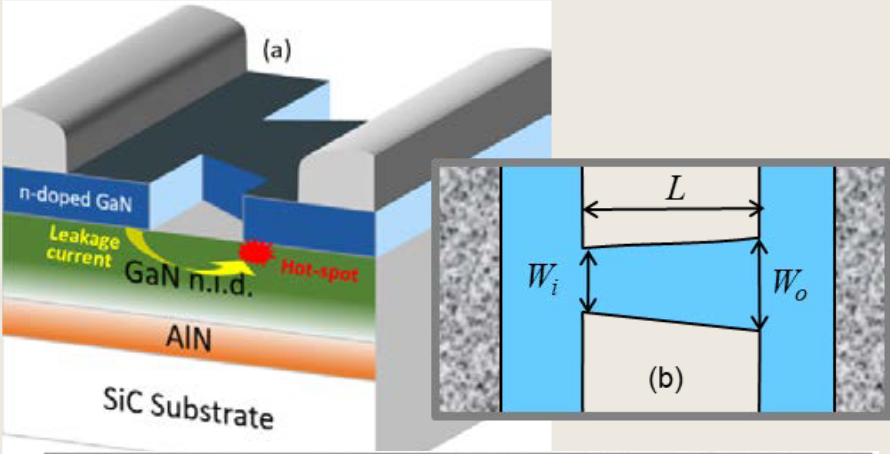
\includegraphics[width=0.9\textwidth]{pa1.png}
    \caption{异形沟道几何结构}
\end{figure}

\clearpage
\subsection{提出的新型设计}

\subsubsection{设计动机：解决“雪崩先于振荡”的核心瓶颈}

上述"异形沟道"方案虽然巧妙，但并未从根本上解决问题。深入研究发现，这种GS-PGD（异形沟道平面耕氏二极管）器件\textbf{依然会失效}，并且通过对比脉冲和直流测试（如下图所示），证明了失效\textbf{并非由自热效应引起}。

\begin{figure}[H]
    \centering
    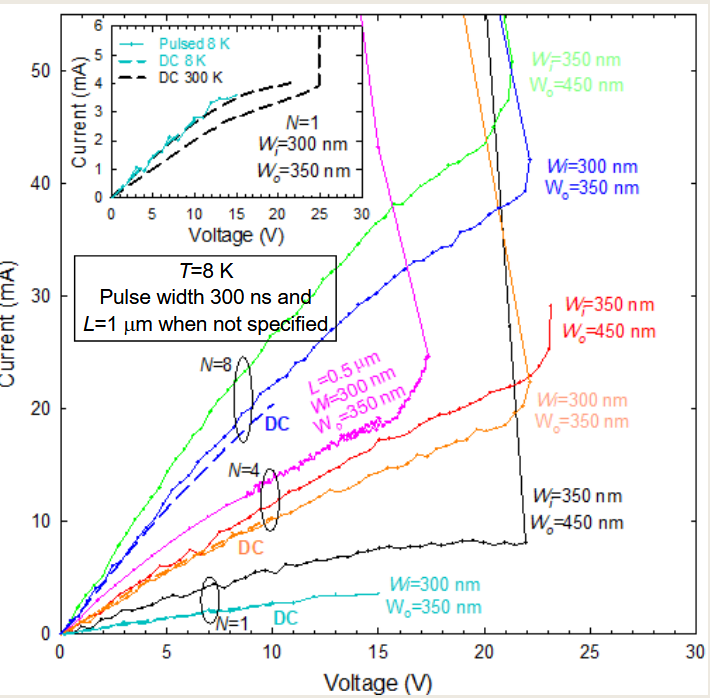
\includegraphics[width=0.6\textwidth]{pa2.png}
    \caption{脉冲与直流测试对比}
\end{figure}


该团队\cite{2024guideline}定位了真正的“杀手”：失效发生在沟道电场达到约 200 kV/cm 时，这恰好是GaN的NDR阈值。3D仿真揭示了真相：在器件绝缘沟槽（trench）的\textbf{阳极（Anode）侧底部角落}，存在一个电场“热点”（Hot Spot）。同时，总有电子\textbf{从沟槽下方“泄露”过去}（Leaked electrons）。当耕氏域形成时，这个局部的超高电场热点会触发泄露电子，导致\textbf{雪崩效应（avalanche process）}，从而在器件达到稳定振荡之前就\textbf{灾难性地烧毁了}。

\clearpage
\subsubsection{设计结构：三端异形沟道平面耕氏二极管 (3T-GS-PGD)}

为了从根本上解决这个“雪崩先于振荡”的核心难点，我们基于文献的启发，提出一种创新的基于自对准阳极场板的三端异形沟道平面耕氏二极管（3T-GS-PGD: Three-Terminal Geometrically-Shaped Planar Gunn Diode）。

对于三端异形沟道平面耕氏二极管（3T-GS-PGD），该设计在保留横向平面型（Lateral Device）拓扑和T型沟道几何优势的基础上，做出了关键性的革新：
在传统的阴极（Source）和阳极（Drain）之外，我们通过器件底部挖槽和金属沉积，引入了\textbf{第三个电极——衘底控制端（$V_S$）}。该电极与有源层下方的缓冲层或衘底相接触。

\begin{figure}[H]
    \centering
    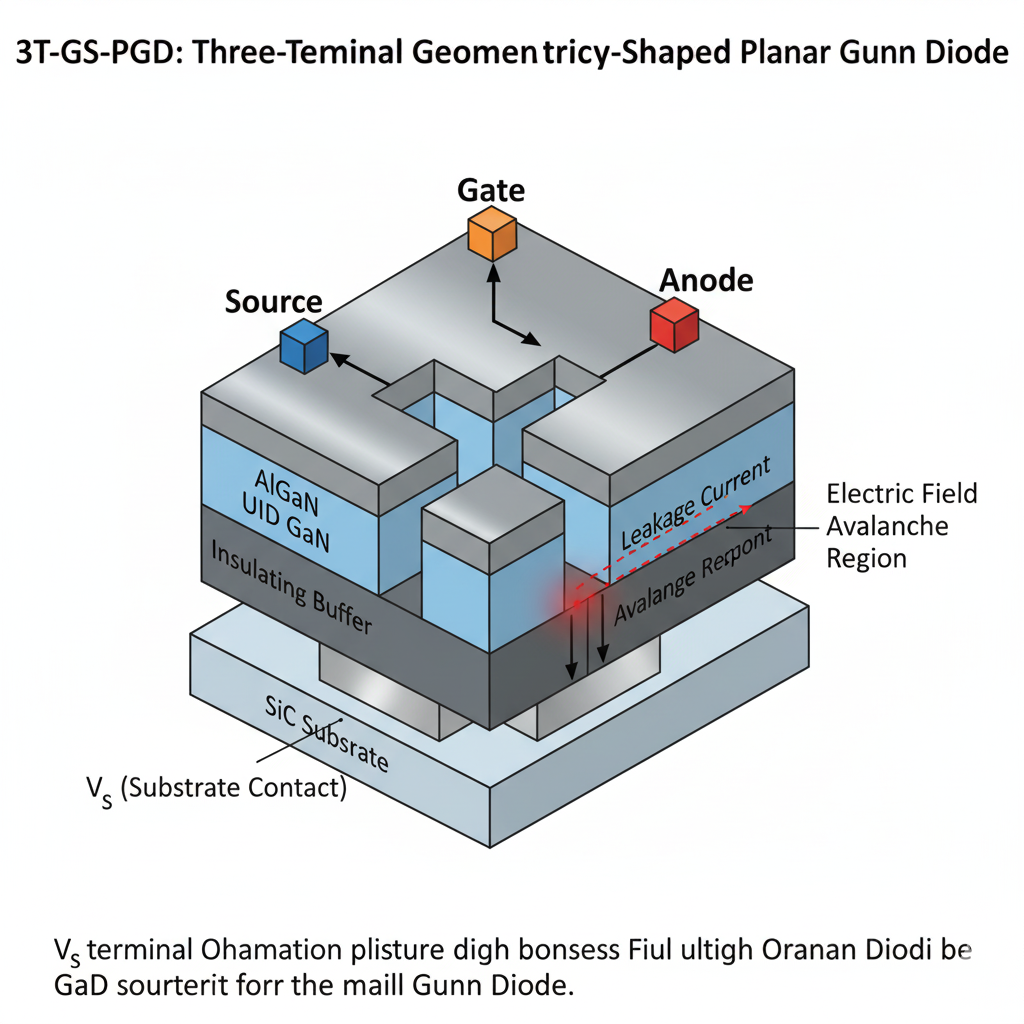
\includegraphics[width=0.5\textwidth]{design.png}
    \caption{3T-GS-PGD结构示意图}
\end{figure}

这个新增的 $V_S$ 端提供了一个\textbf{“正交”的控制维度}，其唯一目的就是\textbf{主动抑制雪崩击穿}，从而“保护”耕氏振荡的发生。如下图所示，通过调控 $V_S$ 电压，冲击电离率可以被\textbf{极大地抑制}：

\begin{figure}[H]
    \centering
    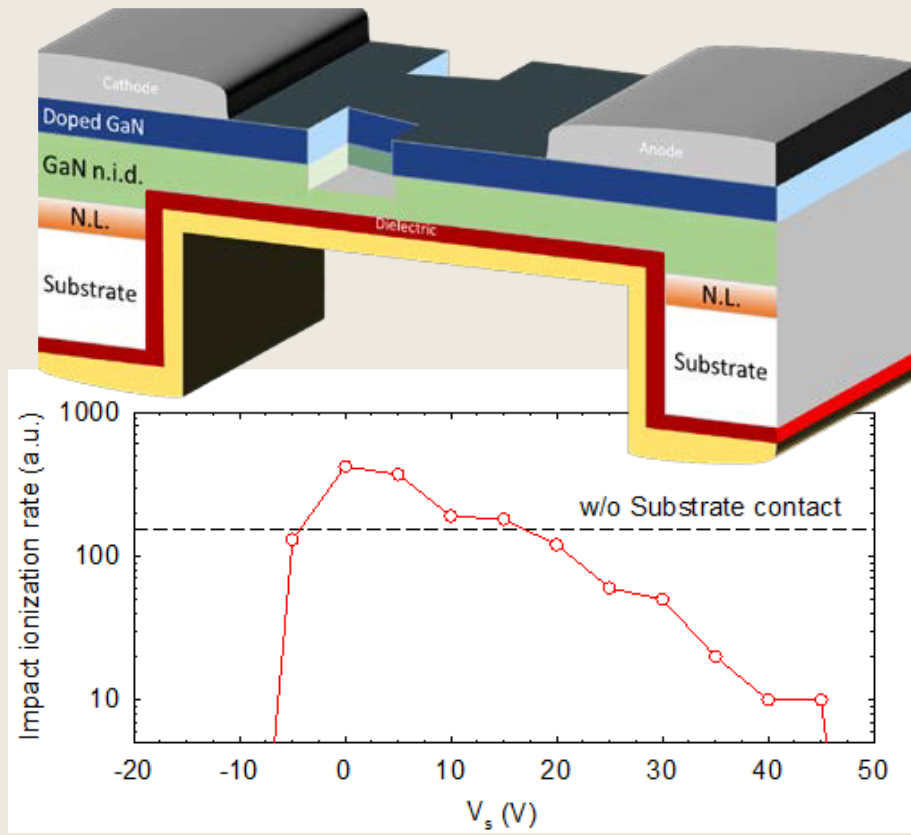
\includegraphics[width=0.4\textwidth]{pa3.png}
    \caption{调控$V_S$电压对冲击电离率的抑制效果}
\end{figure}

\begin{enumerate}
    \item \textbf{主动抑制漏电流（施加负偏压 $V_S < 0$）：}
    通过对 $V_S$ 施加一个\textbf{负偏压}（相对于阴极），可以在有源沟道下方形成一个耗尽区。这如同一个场效应管的栅极，能有效“夹断”沟槽下方的泄露电流路径，从源头上杜绝了引发雪崩的“种子”电子。

    \item \textbf{电场热点整形（施加正偏压 $V_S > 0$）：}
    通过对 $V_S$ 施加一个\textbf{正偏压}（例如，将其与阳极短接），可以主动抬高沟槽底部的电势，有效\textbf{平滑和抑制}阳极侧角落的电场热点，使其峰值远低于触发冲击电离所需的阈值电场（GaN 约 3.3 MV/cm）。
\end{enumerate}

这种三端设计，将“高场振荡”（由源-漏电压 $V_{DS}$ 控制）和“雪崩抑制”（由衬底电压 $V_S$ 控制）这两个在两端器件中相互冲突的物理过程成功\textbf{“解耦”}（Decouple），从而保证器件能安全地工作在耿氏振荡区。

尽管3T-GS-PGD在电学上解决了击穿问题，但其三维结构给制造和高频（THz）信号提取带来了新的挑战。该设计需要"底部挖槽"（bottom recess）和"沉积薄电介质"，这在工艺上非常复杂。为此，我们提出一种优化方案，使设计更趋完美。

\subsubsection{优化方案：自对准阳极场板（Self-Aligned Anode Field Plate）}

作为一种"无源"的替代或补充方案，自对准阳极场板技术能够从根本上消除电场热点。在制造T型沟道时，采用自对准工艺，使阳极金属通过一层介质\textbf{延伸并覆盖在阳极侧的沟槽边缘之上}，形成"场板"（Field Plate）结构。

这种设计具有三方面的显著优势。首先，在\textbf{电场整形}方面，场板的"帽子"效应可以有效平滑电场分布，\textbf{从根本上消除}阳极侧沟槽边缘的电场热点，避免局部电场过度集中引发的击穿问题。其次，在\textbf{简化设计}方面，这种方法有可能\textbf{不再需要 3T-GS-PGD 的第三个衬底端子}，使器件回归到更简单的两端结构，极大地降低了制造难度和寄生效应，提高了器件的可靠性和制造成品率。最后，在\textbf{兼容性}方面，即使场板不能完全消除雪崩，它也可以大大降低对 $V_S$ 偏压的要求，与3T-GS-PGD方案\textbf{完全兼容}，使其工作更加稳定，为器件设计提供了更大的灵活性。

通过这种优化方案，我们既保留了3T-GS-PGD的雪崩抑制能力，又简化了制造工艺，为实现高性能GaN耿氏二极管提供了一条更加实用的技术路径。

\subsubsection{参数设计}

本设计的目标是实现THz频段（具体目标 $f > 300$ GHz）的稳定振荡，并克服GaN器件中"雪崩先于振荡"的核心瓶颈。

\textbf{1. 材料与导电类型选择}

选用氮化镓（GaN）作为有源材料，导电类型为n型半导体。GaN具有 $2.7 \times 10^7$ cm/s的高电子饱和速度和3.3 MV/cm的高击穿场强，远优于GaAs，是实现高功率和高频率振荡的理想材料。器件结构基于 $n^+/n/n^+$ 掺杂方案。

\textbf{2. 工作电场选定}

根据文献及仿真分析，GaN的负微分电导（NDR）区域约在电场 $E > 200$ kV/cm时开始。为激发耿氏效应，有源区内的电场必须高于此阈值。我们设计的T型沟道会在阴极附近"聚焦"电场，器件的平均工作电场 $E_{\text{avg}}$ 设定为250 kV/cm，确保器件稳定工作在NDR区。在T型沟道的最窄处（高场区），电场会远高于此平均值，以有效触发和"钉扎"耿氏畴的形成。

\textbf{3. 畴区移动速度}

采用GaN的电子饱和速度 $v_d$ 作为畴区移动速度 $v_s$，选定值为 $v_s \approx 2.7 \times 10^7$ cm/s。

\textbf{4. 沟道长度确定}

对于平面型（Lateral Device）设计，关键参数L对应的是沟道长度（Channel Length）。设计目标为 $f = 500$ GHz。根据渡越时间振荡公式 $f \approx v_s / L$：

\begin{equation}
L \approx \frac{v_s}{f} = \frac{2.7 \times 10^7 \text{ cm/s}}{500 \times 10^9 \text{ Hz}} = 0.54 \text{ µm}
\end{equation}

为便于制造，选定有源区的沟道长度 $L = 0.5$ µm (500 nm)。

\textbf{5. 工作电压估算}

根据物理关系 $V = E \times L$：

\begin{equation}
V = E_{\text{avg}} \times L = (250 \text{ kV/cm}) \times (0.5 \times 10^{-4} \text{ cm}) = 12.5 \text{ V}
\end{equation}

预计启动电压和工作电压V在10 V到20 V之间。这个电压远低于GaN的理论击穿电压，验证了T型沟道设计在降低工作电压上的有效性。

\textbf{6. 掺杂设计}

遵循 $n^+/n/n^+$ 的掺杂结构。有源区（n-GaN）采用"掺杂GaN"方案，掺杂浓度需满足Kroemer准则 $n_0L > 10^{13}$ cm$^{-2}$：

\begin{equation}
n_0 > \frac{10^{13} \text{ cm}^{-2}}{0.5 \times 10^{-4} \text{ cm}} = 2 \times 10^{17} \text{ cm}^{-3}
\end{equation}

为确保畴的快速形成，选择 $N_D \approx 1 \times 10^{18}$ cm$^{-3}$。过渡区（$n^+$-GaN）用于连接金属电极，实现低电阻欧姆接触，选定为 $N_D > 5 \times 10^{19}$ cm$^{-3}$。

\textbf{7. 电极引出方式}

采用3T-GS-PGD的三电极结构。阴极和阳极采用平面型（Lateral）结构，电极（如Ti/Al/Ni/Au）沉积在器件顶部的 $n^+$-GaN过渡区上。第三电极 $V_S$（衬底控制端）通过在SiC衬底上进行底部挖槽（bottom recess）并沉积金属，从器件底部引出。该电极用于施加控制偏压 $V_S$，主动抑制漏电流和电场热点。

\begin{table}[H]
    \centering
    \caption{3T-GS-PGD关键设计参数}
    \begin{tabular}{p{4.5cm}p{3.5cm}p{5.5cm}}
        \toprule
        \textbf{参数} & \textbf{设计值} & \textbf{说明} \\
        \midrule
        材料 & GaN（n型） & 高饱和速度、高击穿场强 \\
        沟道长度 (L) & 0.5 µm (500 nm) & 实现500 GHz目标频率 \\
        平均工作电场 ($E_{\text{avg}}$) & 250 kV/cm & 稳定工作在NDR区 \\
        畴区移动速度 ($v_s$) & $2.7 \times 10^7$ cm/s & 采用GaN饱和速度 \\
        工作电压 (V) & 10--20 V & T型沟道降低启动电压 \\
        有源区掺杂 ($N_D$) & $1 \times 10^{18}$ cm$^{-3}$ & 满足Kroemer准则 \\
        过渡区掺杂 ($N_D^+$) & $> 5 \times 10^{19}$ cm$^{-3}$ & 实现良好欧姆接触 \\
        电极结构 & 三端（3T） & 阴极、阳极、衬底控制端 \\
        目标振荡频率 & > 300 GHz & 进入THz频段 \\
        \bottomrule
    \end{tabular}
\end{table}

\clearpage

\section{生产安全防护考虑}

本设计采用GaN（氮化镓）作为有源层材料，SiC（碳化硅）作为衬底。

\subsection{材料本身安全性}

与GaAs（砷化镓）不同，GaN和SiC的最终晶体材料化学性质极其稳定，被认为是生物相容和无毒的。因此，器件在使用和废弃阶段，因材料本身毒性（如砷As）所带来的安全风险极低。

\subsection{生产制造过程中的安全防护}

\subsubsection{剧毒及易燃易爆气体防护}

GaN的MOCVD外延生长是主要风险点。

\emph{危害辨识：} 此过程需使用三甲基镓（TMGa）等金属有机源（MO源）和氨气（NH$_3$）。TMGa是一种自燃性液体，其蒸气遇空气即自发燃烧爆炸；NH$_3$则是剧毒、腐蚀性气体。

\emph{防护措施：} 必须配备双层套管的特气输送系统、交叉锁定的安全控制面板、实时的气体侦测器及报警器（类比指导文件中的砷化氢/氧化砷侦测器），并配备紧急火灾抑制系统。

\subsubsection{强酸腐蚀防护}

\emph{危害辨识：} T型沟道的干法或湿法刻蚀工序，以及光刻胶去除等步骤，会使用氢氟酸（HF）、硫酸（H$_2$SO$_4$）、硝酸（HNO$_3$）等强酸和强氧化剂。

\emph{防护措施：} 刻蚀工序必须在配备专业抽风系统的通风橱（Fume Hood）中进行。操作人员必须佩戴防酸面罩、厚制防化手套和防腐蚀工作服。必须常备葡萄糖酸钙凝胶作为HF烧伤的紧急中和剂。

\subsubsection{人员安全与培训}

\emph{防护措施：} 必须严格遵守指导文件中的原则：制定严格的操作规范与事故处理预案，做好安全防护与安全教育，进行危害辨识、认知与预防的训练。同时，应定期对员工进行职业健康体检（类比血砷含量体检），确保操作人员健康与安全。

\clearpage

\section{社会与环境因素评估}

\subsection{环境影响}

\subsubsection{材料与废弃物}

GaN和SiC材料本身稳定无毒，废弃器件对土壤和水源的直接化学污染风险远低于GaAs器件（因其含As）。

\subsubsection{生产废弃物}

最大的环境挑战在于生产过程。MOCVD的气体利用率并非100\%，大量未反应的NH$_3$和有机金属化合物会随尾气排出。此外，刻蚀和清洗工序会产生大量的酸性废水和有机溶剂废液。

\emph{处理措施：} 必须配备高效的尾气处理系统（Scrubber），对剧毒和自燃性气体进行燃烧或化学中和处理。必须建立配套的废水处理站，对酸碱废液进行中和，并去除重金属离子，确保所有排污符合环保标准，不对空气、水资源、土壤产生影响。

\subsection{社会影响}

\subsubsection{能源消耗与可持续性}

GaN和SiC的外延生长（MOCVD或高温CVD）均需要在超过1000$^{\circ}$C的高温下进行，是一个高能耗过程。从全生命周期看，器件制造阶段的碳足迹较高。

\subsubsection{积极的社会效益}

必须强调，这种"前期高投入"是为了实现"后期高效益"。GaN是第三代半导体的核心，其在功率转换上的高效率（远超传统硅基器件）正在极大地降低全球数据中心、充电桩和电网的整体能耗。

\subsubsection{技术应用伦理}

本3T-GS-PGD设计所针对的THz领域，是6G通信、高分辨率医疗成像（如皮肤癌早期检测）和公共安全（无辐射安检）的核心技术。这些应用能极大地推动科技进步、增进人类福祉，符合社会发展的积极方向，不存在已知的道德、法律或风俗问题。

\clearpage

\section{总结}

本设计针对 THz 固态振荡源需求，提出基于自对准阳极场板的三端异形沟道平面耿氏二极管（3T-GS-PGD）。

\subsection{核心创新}

传统GaN耿氏二极管因阳极侧沟槽边缘电场热点触发泄露电子雪崩而失效。本设计通过\textbf{自对准阳极场板}从根本上消除该热点；配合\textbf{底部控制极$V_S$}（负偏压夹断漏电流、正偏压平滑电场）与\textbf{T型沟道}（降低启动电压至10--20 V），实现高场振荡与雪崩抑制的安全解耦，确保器件在亚微米沟道下稳定工作于>300 GHz。

\subsection{关键设计参数}

本设计充分利用GaN材料优势（高饱和速度$2.7 \times 10^7$ cm/s、高击穿场强3.3 MV/cm），通过系统化参数设计实现THz目标：

\begin{itemize}
    \item \textbf{有源层：}采用掺杂GaN方案（$n^+/n/n^+$结构），有源区掺杂$N_D \approx 1 \times 10^{18}$ cm$^{-3}$，满足Kroemer准则$n_0L > 10^{13}$ cm$^{-2}$。
    \item \textbf{沟道长度：}$L = 0.5$ µm（500 nm），根据渡越时间公式$f = v_s / L$实现目标频率$f = 500$ GHz。
    \item \textbf{工作电场：}平均工作电场$E_{\text{avg}} = 250$ kV/cm，确保稳定工作在NDR区。
    \item \textbf{热管理：}采用SiC衬底（热导率4.9 W/cm·K），有效缓解自热效应。
\end{itemize}

\subsection{工程实施与安全评估}

本设计全面考虑了工程实际问题：

\textbf{制造工艺：}基于成熟的MOCVD外延生长、光刻刻蚀（T型沟道）、金属沉积（Ti/Al/Ni/Au电极）和底部挖槽（第三电极引出）技术，工艺路线清晰可行。

\textbf{安全防护：}针对MOCVD过程中的剧毒气体（TMGa自燃、NH$_3$剧毒）和刻蚀工序中的强酸（HF、H$_2$SO$_4$），制定了完备的危害辨识、防护措施（双层套管、气体侦测、通风橱、防化装备）和人员培训方案。

\textbf{环境影响：}GaN和SiC材料本身无毒稳定，优于GaAs器件。生产过程需配备尾气处理系统（Scrubber）和废水处理站，确保排污符合环保标准。虽然外延生长高能耗（>1000$^{\circ}$C），但GaN器件的高效率特性能在全生命周期实现"后期高效益"，符合可持续发展原则。

\subsection{应用前景与社会价值}

本3T-GS-PGD设计突破了GaN耿氏二极管的核心技术瓶颈，为THz固态振荡源提供了可行的工程化路径。其应用领域包括：

\begin{itemize}
    \item \textbf{6G无线通信：}THz频段高速数据传输（Tbps级）。
    \item \textbf{医疗成像：}高分辨率非侵入式检测（如皮肤癌早期诊断）。
    \item \textbf{公共安全：}无辐射安检（检测隐藏武器和爆炸物）。
    \item \textbf{航空航天：}高精度遥感和大气监测。
\end{itemize}

这些应用将极大推动科技进步和人类福祉，具有显著的社会价值和经济效益。

\subsection{结论}

本设计基于自对准阳极场板的3T-GS-PGD方案，突破GaN耿氏器件"雪崩先于振荡"瓶颈，实现10--20 V启动、>300 GHz稳定振荡。方案兼顾电学性能、工艺可行性与安全环保要求，为室温THz固态振荡源提供完整技术路径，具有重要科学意义与产业转化潜力。

\clearpage
\bibliographystyle{IEEEtran}
\begin{thebibliography}{9}

\bibitem{tonouchi2007cutting}
M. Tonouchi, ``Cutting-edge terahertz technology,'' \emph{Nature Photon.}, vol. 1, pp. 97--105, Oct. 2007.

\bibitem{siegel2004terahertz}
P. H. Siegel, ``Terahertz technology in biology and medicine,'' in \emph{IEEE MTT-S Int. Microw. Symp. Dig.}, Jun. 2004, pp. 1575--1578.

\bibitem{belkin2007terahertz}
M. A. Belkin et al., ``Terahertz quantum-cascade-laser source based on intracavity difference-frequency generation,'' \emph{Nature Photon.}, vol. 1, no. 5, pp. 288--292, 2007.

\bibitem{suzuki1995first}
M. Suzuki, T. Uenoyama, and A. Yanase, ``First-principles calculations of effective mass parameters of AlN and GaN,'' \emph{Physical Review B}, vol. 52, no. 11, p. 8132, 1995.

\bibitem{yao2014thz}
姚慧, ``THz 波段 GaN 耕氏二极管非线性模型及振荡器研究,'' 硕士学位论文, 西安电子科技大学, 2014.

\bibitem{li2018gan}
李玉梅, ``GaN 基太赫兹耿氏二极管结构及工艺研究,'' 硕士学位论文, 西安电子科技大学, 2018.

\bibitem{chowdhury2013lateral}
S. Chowdhury and U. K. Mishra, ``Lateral and vertical transistors using the AlGaN/GaN heterostructure,'' \emph{IEEE Transactions on Electron Devices}, vol. 60, no. 10, pp. 3060--3066, Oct. 2013.

\bibitem{2024guideline}
J. Mateos et al., "Guidelines for Overcoming the Practical Limitations for the Fabrication of THz Sources with GaN Planar Gunn Diodes," in \emph{2024 8th IEEE Electron Devices Technology \& Manufacturing Conference (EDTM)}, 2024, pp. 1--3.

\end{thebibliography}

\end{document}